\def\micro{\mu m}
\def\um{$\micro$ }
\def\degreesC{$\degree C$ }
\def\percent{$\%$ }
\documentclass[10pt,a4paper,oneside]{article}
\usepackage[left=2cm,right=2cm,top=2cm,bottom=2cm]{geometry}

\usepackage[dvipsnames]{xcolor}

%%  -------------------------------------------------------------------
%%      GDS II layer, regarding MOSIS SCMOS layer map
%%  -------------------------------------------------------------------
% GDS II #41 - P_WELL
\definecolor{pwell}{rgb}{1.0, 0.74, 0.53}   % macaroni and cheese
% GDS II #42 - N_WELL
\definecolor{nwell}{rgb}{0.61, 0.87, 1.0}  % columbia blue
\definecolor{pbase}{rgb}{1.0, 0.51, 0.26}  % mango tango
\definecolor{nbase}{rgb}{0.0, 0.75, 1.0}   % capri 
% GDS II #43 - ACITVE
\definecolor{active}{rgb}{0.9, 0.4, 0.38}   % light carmine pink
% GDS II #45 - N_PLUS_SELECT
\definecolor{nimplant}{rgb}{0.45, 0.76, 0.983}% maya blue
% GDS II #44 - P_PLUS_SELECT
\definecolor{pimplant}{rgb}{1.0, 0.51, 0.26}% mango tango
% GDS II #46 - POLY
\definecolor{poly}{rgb}{0.56, 0.93, 0.56}   % light green
% GDS II #25 - CONTACT
\definecolor{contact}{rgb}{0.83, 0.83, 0.83}% light gray
% GDS II #49 - METAL1
\definecolor{metal1}{rgb}{0.38, 0.31, 0.86} % majorelle blue
% GDS II #50 - VIA1
\definecolor{via1}{rgb}{0.83, 0.83, 0.83}   % light gray
% GDS II #51 - METAL2
\definecolor{metal2}{rgb}{0.04, 0.85, 0.32} % malachite
% GDS II #61 - VIA2
\definecolor{via2}{rgb}{0.83, 0.83, 0.83}   % light gray
% GDS II #63 - METAL3
\definecolor{metal3}{rgb}{0.98, 0.93, 0.37} % maize
% GDS II #30 - VIA3
\definecolor{via3}{rgb}{0.83, 0.83, 0.83}   % light gray
% GDS II #31 - METAL4
\definecolor{metal4}{rgb}{0.75, 0.25, 0.0}  % mahogany
% GDS II #32 - VIA4
\definecolor{via4}{rgb}{0.83, 0.83, 0.83}   % light gray
% GDS II #33 - METAL5
\definecolor{metal5}{rgb}{0.79, 0.08, 0.48} % magenta (dye)
% GDS II #36 - VIA5
\definecolor{via5}{rgb}{0.83, 0.83, 0.83}   % light gray
% GDS II #37 - METAL6
\definecolor{metal6}{rgb}{0.11, 0.35, 0.02} % lincoln green
% GDS II #29 - SILICIDE_BLOCK
\definecolor{silicide-block}{rgb}{0.98, 0.94, 0.9}  % linen
% GDS II #52 - GLASS
\definecolor{glass}{rgb}{1.0, 1.0, 0.88}    % light yellow
% GDS II #26 - PADS
\definecolor{pads}{rgb}{0.75, 1.0, 0.0}     % lime (color wheel)

\definecolor{resist}{rgb}{0.71, 0.4, 0.11}  % light brown

\definecolor{silicide}{rgb}{0.29, 0.33, 0.13}
\definecolor{titanium}{rgb}{0.8, 0.58, 0.46}

\def\OpacityLayout {0.5}

%
% physical
%
\definecolor{substrate}{rgb}{0.96, 0.94, 0.93}  % isabelline
\definecolor{nitride}{rgb}{1.0, 0.03, 0.0}
\definecolor{gateoxide}{rgb}{0.88, 1.0, 1.0}    % light cyan
\definecolor{isolationoxide}{rgb}{0.84, 0.79, 0.87}% languid lavender

\usepackage[utf8]{inputenc}
\usepackage[english]{babel}
\usepackage{forloop}
\usepackage{amsmath}
\usepackage{amsfonts}
\usepackage{amssymb}
\usepackage{gensymb}
\usepackage{mdframed}
\usepackage{graphicx}
\usepackage{tikz}
\usetikzlibrary{arrows,automata,shapes}
\usepackage[siunitx]{circuitikz}
\usepackage{makecell}
\usepackage{array}

\def\WaferClean{
\begin{tikzpicture}\node [fill=cyan, rounded corners=5pt] {\large Clean};\end{tikzpicture}}
\def\WaferSemiClean{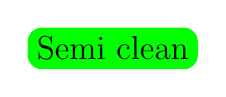
\begin{tikzpicture}\node [fill=green, rounded corners=5pt] {\large Semi clean};\end{tikzpicture}}
\def\WaferNonStandard{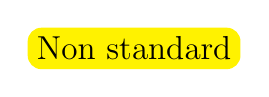
\begin{tikzpicture}\node [fill=yellow, rounded corners=5pt] {\large Non standard};\end{tikzpicture}}

\usepackage[colorlinks=true,linkcolor=blue,urlcolor=black,bookmarksopen=true]{hyperref}
\usepackage{bookmark}
\usepackage{hyperref}
\usepackage{sepfootnotes}
\usepackage{lipsum,tocloft} 
\usetikzlibrary{positioning}
\usetikzlibrary{patterns}

\usepackage{float}
\floatstyle{boxed} 
\restylefloat{figure}

\title{Libre Silicon process testing}
\date{\today}
\author{David Lanzendörfer}
\makeindex

\newcounter{ct}
\def\CrossSectionOnly{0.3}
\def\CrossAndTopSection{0.2}
\def\CrossAndTopSectionBig{0.3}
\def\VLSILayout{0.4}

\DeclareMathOperator\erfc{erfc}

\setlength{\parindent}{0pt} % get rid of annoying indents

\begin{document}
\begin{abstract}
	Copyright © 2017 LANCEVILLE TECHNOLOGY GROUP CO., LIMITED. All rights reserved. \\

This process is licensed under the Libre Silicon public license; you can redistribute it and/or modify it under the terms of the Libre Silicon public license
as published by the Libre Silicon alliance, either version 1 of the License, or (at your option) any later version.

This design is distributed in the hope that it will be useful, but WITHOUT ANY WARRANTY; without even the implied warranty of MERCHANTABILITY or FITNESS FOR A PARTICULAR PURPOSE.
See the Libre Silicon Public License for more details. \\

This document is part of the specification of the free silicon manufacturing standard for manufacturing the LibreSilicon standard logic cells\footnote{\url{https://github.com/chipforge/StdCellLib}} and related free technology nodes from the LibreSilicon project.

For this initial revision 0.1 a gate-first approach has been chosen which led to the choice of polysilicon as the gate electrode material because of the simplicity of the gate alignment.
For better isolation properties of the transistors and gates in overall a box-isolation approach has been chosen.
All of these choices have been made with the future scale down from the recent $1 \mu m$ to smaller structure sizes.
\textbf{This process is for manufacturing $1 \mu m$ only!}
But further releases which will have been tested with smaller structure sizes can be expected.

\end{abstract}

\newpage
\tableofcontents

\maketitle
In order to get an idea on how strongly the actual product differs from the mathematical models being used before hand to define the initial parameters, one has to run a bunch of test wafers through the process over and over again, tweak parameters and measure out all kinds of aspects of the device.

This is also important for gathering the data which will finally end up within the data sheet.

In this chapter we will tackle the multiple different measurement and test objects we will need to put into the seal area during production in order to ensure the consistent quality of the chips we're going to sell in the end.\\



\textbf{Testing parameters:}
\begin{itemize}
	\item Passive properties:
	\begin{itemize}
		\item The capacity per $m^2$ from the n-well to the gate electrode
		\item The capacity per $m^2$ from  the p-well to the gate electrode
		\item The actual resistance/m of the p-well
		\item The actual resistance/m of the n-well
		\item The actual resistance/m of the p-implant layer
		\item The actual resistance/m of the n-implant layer
		\item The actual resistance/m of the poly layer
		\item The actual resistance/m of the silicide+p-implant layer
		\item The actual resistance/m of the silicide+n-implant layer
		\item The actual resistance/m of the silicide+poly layer
	\end{itemize}

	\item Diodes:
	\begin{itemize}
		\item ESD structure diodes (Voltage protection)
		\item Lateral diodes
		\item Vertical diodes
	\end{itemize}

	\item Bipolar transistors:
	\begin{itemize}
		\item Vertical bipolar transistor (to test latchup conditions)
		\item Lateral bipolar transistors (to see what the beta is)
	\end{itemize}

	\item NMOS as well as PMOS:
	\begin{itemize}
		\item Frequency characteristics (Transient curve)
		\item Drain-source resistance vs. gate-source voltage
		\item Actual threshold voltage
	\end{itemize}
\end{itemize}

Each of these values will variate based on the location on the wafer, because of diffraction towards the edge and also because of the uneven nature of the wafer.

Measuring the same test structure multiple times placed at multiple locations on the wafer will allow us to calculate an effective average value and tolerance ranges for taking into account for further dimensioning of circuits..

\newpage
\section{Diodes}
There are multiple different diode types possible which could form, which can be categorized into two categories: Lateral and vertical.

Lateral diodes can form between two wells or the well and the junction, the vertical diodes can form between the n-well and the p-substrate.

\subsection{Lateral diodes}

\begin{figure}[H]
	\centering
	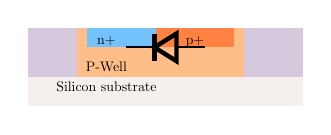
\begin{tikzpicture}[node distance = 3cm, auto, thick,scale=0.5, every node/.style={transform shape}]
		% substrate
\fill[substrate] (0,0) rectangle (7,2);
\node at (2,0.5) {Silicon substrate};
%trenches
\fill[isolationoxide] (0,0.75) rectangle (1.25,2);
\fill[isolationoxide] (5.5,0.75) rectangle (7,2);
% p-well
\fill[pwell] (1.25,0.75) rectangle (5.5,2);
\node at (2,1) {P-Well};

\fill[nimplant] (1.5,1.5) rectangle (3.5,2);
\node at (2,1.65) {n+};
\fill[pimplant] (3.25,1.5) rectangle (5.25,2);
\node at (4.25,1.65) {p+};

\draw (4.5,1.5) to[D,n=diode] (2.5,1.5);
	\end{tikzpicture}
	\caption{Lateral diode cross section}
	\label{lateral_diode_cross_section}
\end{figure}

\subsection{Vertical diodes}

\begin{figure}[H]
	\centering
	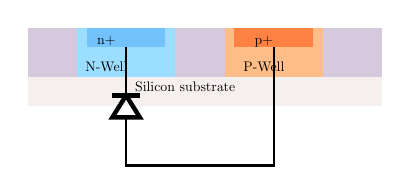
\begin{tikzpicture}[node distance = 3cm, auto, thick,scale=0.5, every node/.style={transform shape}]
		% substrate
\fill[substrate] (0,0) rectangle (9,2);
\node at (4,0.5) {Silicon substrate};
%trenches
\fill[isolationoxide] (0,0.75) rectangle (1.25,2);
\fill[isolationoxide] (3.75,0.75) rectangle (5,2);
\fill[isolationoxide] (7.5,0.75) rectangle (9,2);

% n-well
\fill[nwell] (1.25,0.75) rectangle (3.75,2);
\node at (2,1) {N-Well};
\fill[nimplant] (1.5,1.5) rectangle (3.5,2);
\node at (2,1.65) {n+};

% p-well
\fill[pwell] (5,0.75) rectangle (7.5,2);
\node at (6,1) {P-Well};
\fill[pimplant] (5.25,1.5) rectangle (7.25,2);
\node at (6,1.65) {p+};

\draw (6.25,1.5) -- (6.25,-1.5) -- (2.5,-1.5) to[D,n=diode] (2.5,1.5);

	\end{tikzpicture}
	\caption{Vertical diode cross section}
	\label{vertical_diode_cross_section}
\end{figure}

\newpage
\subsection{Bipolar transistors}
\newpage
\section{ESD circuit test}

\subsection{ESD diode on p-substrate}
\begin{figure}[H]
	\centering
	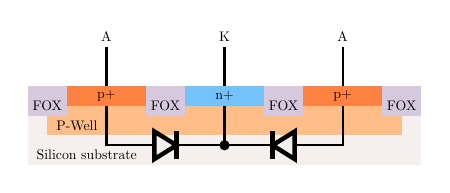
\begin{tikzpicture}[node distance = 3cm, auto, thick,scale=0.5, every node/.style={transform shape}]
		% substrate
\fill[substrate] (0,0) rectangle (10,2);
\node at (1.5,0.25) {Silicon substrate};

% p-well
\fill[pwell] (0.5,0.75) rectangle (9.5,2);
\node at (1.25,1) {P-Well};

%trenches
\fill[isolationoxide] (0,1.25) rectangle (1,2);
\node at (0.5,1.5) {FOX};
\fill[isolationoxide] (3,1.25) rectangle (4,2);
\node at (3.5,1.5) {FOX};
\fill[isolationoxide] (6,1.25) rectangle (7,2);
\node at (6.5,1.5) {FOX};
\fill[isolationoxide] (9,1.25) rectangle (10,2);
\node at (9.5,1.5) {FOX};

\fill[pimplant] (1,1.5) rectangle (3,2);
\node at (2.0,1.75) {p+};
\fill[nimplant] (4,1.5) rectangle (6,2);
\node at (5.0,1.75) {n+};
\fill[pimplant] (7,1.5) rectangle (9,2);
\node at (8.0,1.75) {p+};

\draw (2.0,1.5) -- (2.0,0.5) to[D,n=diode] (5.0,0.5) -- (5.0,1.5);
\draw (8.0,1.5) -- (8.0,0.5) to[D,n=diode] (5.0,0.5) --  (5.0,1.5);

\filldraw (5.0,0.5) circle (0.1);

\draw (2.0,2.0) -- (2.0,3.0);
\node at (2.0,3.25) {A};
\draw (5.0,2.0) -- (5.0,3.0);
\node at (5.0,3.25) {K};
\draw (8.0,2.0) -- (8.0,3.0);
\node at (8.0,3.25) {A};
	\end{tikzpicture}
	\caption{ESD diode on p-substrate cross section}
	\label{p_sub_ESD_cross}
\end{figure}

\subsection{ESD diode on n-substrate}
\begin{figure}[H]
	\centering
	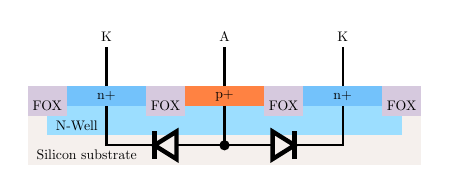
\begin{tikzpicture}[node distance = 3cm, auto, thick,scale=0.5, every node/.style={transform shape}]
		% substrate
\fill[substrate] (0,0) rectangle (10,2);
\node at (1.5,0.25) {Silicon substrate};

% n-well
\fill[nwell] (0.5,0.75) rectangle (9.5,2);
\node at (1.25,1) {N-Well};

%trenches
\fill[isolationoxide] (0,1.25) rectangle (1,2);
\node at (0.5,1.5) {FOX};
\fill[isolationoxide] (3,1.25) rectangle (4,2);
\node at (3.5,1.5) {FOX};
\fill[isolationoxide] (6,1.25) rectangle (7,2);
\node at (6.5,1.5) {FOX};
\fill[isolationoxide] (9,1.25) rectangle (10,2);
\node at (9.5,1.5) {FOX};

\fill[nimplant] (1,1.5) rectangle (3,2);
\node at (2.0,1.75) {n+};
\fill[pimplant] (4,1.5) rectangle (6,2);
\node at (5.0,1.75) {p+};
\fill[nimplant] (7,1.5) rectangle (9,2);
\node at (8.0,1.75) {n+};

\draw (5.0,1.5) -- (5.0,0.5) to[D,n=diode] (2.0,0.5) -- (2.0,1.5);
\draw (5.0,1.5) -- (5.0,0.5) to[D,n=diode] (8.0,0.5) -- (8.0,1.5);
\filldraw (5.0,0.5) circle (0.1);

\draw (2.0,2.0) -- (2.0,3.0);
\node at (2.0,3.25) {K};
\draw (5.0,2.0) -- (5.0,3.0);
\node at (5.0,3.25) {A};
\draw (8.0,2.0) -- (8.0,3.0);
\node at (8.0,3.25) {K};
	\end{tikzpicture}
	\caption{ESD diode on n-substrate cross section}
	\label{n_sub_ESD_cross}
\end{figure}

\end{document}